\section{Marco referencial}

	\subsection{Antecedentes}
	
		\subsubsection{yotepresto.com}
		
		{Es una plataforma web encargada de conectar personas que necesitan un préstamo, con personas que quieren prestar su dinero y obtener un buen rendimiento de él, se basa en un comunidad que va depositando su dinero en un fondo, el cual será utilizado por otras personas que lo necesiten, generando intereses o ganancias, las personas que necesiten un préstamo son consultadas en centrales de riesgo para verificar su historial crediticio y capacidad de pago, y posterior a esto realizarse el desembolso de su crédito gracias al fondo de los que invierten \cite{yotepresto}.\\
			
		Si bien yotepresto.com permite gestionar créditos, no se enfoca al mismo negocio planteado en proyecto, pues este pretende suplir la necesidad de los tenderos de vender sus productos por medio de prestamos a sus clientes.\\
		
		\begin{figure}[H]
			\centering
			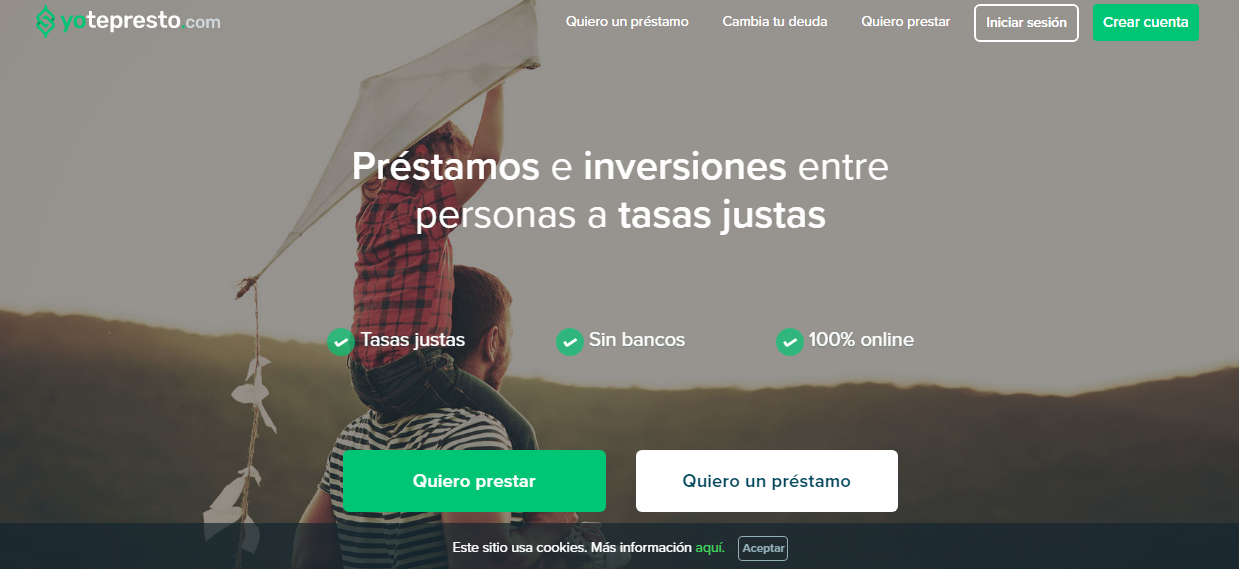
\includegraphics[width=0.8\linewidth]{description/framework/yotepresto.png}
			\caption{Web yotepresto.com}
		\end{figure}
	
		\begin{center}
			\textbf{Fuente:} \url{https://www.yotepresto.com/}
		\end{center}
		}
	
	
	\subsection{Marco teórico}
	
		\subsubsection{Microcrédito}
		
		{Es una fuente de financiación enfocada a los hogares con bajos ingresos, esta, trata de proveer pequeños prestamos impulsando el desarrollo económico de los interesados, permitiendo la adquisición de activos o bienes de bajo costo, es basada en la hipótesis de "para bajar los índices de pobreza es indispensable dar acceso a los recursos financieros" \cite{MaricruzMicro,BarbaraMicro}.\\
		
		El microcrédito, es imprecindible como fuente de financiación para las personas que se encargan a las ventas informales, este permite que sus clientes tengan acceso a sus productos, incrementar el porcentaje de sus ventas y fidelizar a los mismos \cite{LupeTrust}.\\
	
		\begin{figure}[H]
			\centering
			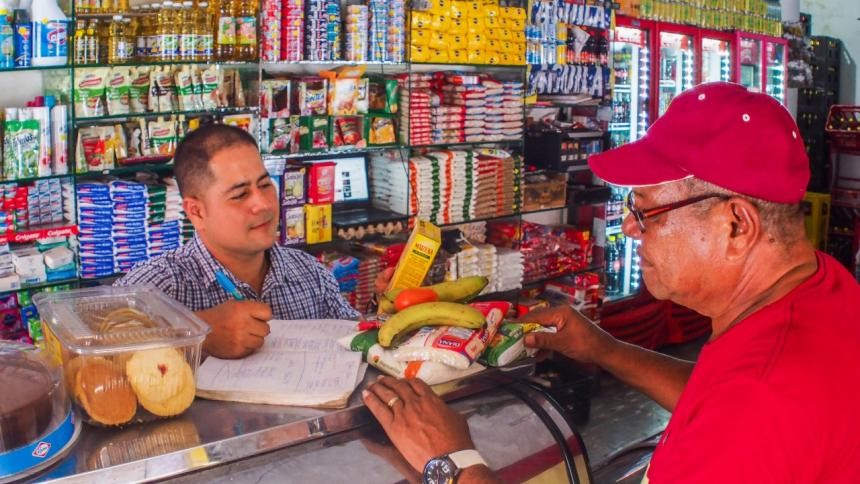
\includegraphics[width=0.8\linewidth]{description/framework/tendero.jpg}
			\caption{Tendero fiando}
		\end{figure}
	
		\begin{center}
			\textbf{Fuente:} \url{https://www.elheraldo.co/economia/el-fiao-el-que-salva-las-tiendas-653295}
		\end{center}
		}
	
	
		\subsubsection{Experiencia de usuario}
		
		{La experiencia de usuario hace referencia a la visión o al diseño en la que el proceso o interactividad de la aplicación, está delimitada o conducida empíricamente por la información recopilada de la audiencia objetivo del producto, esto con el fin de garantizar una navegabilidad fluida entre cada uno de sus usuarios, para esto, es necesario tener en cuenta la “interacción”, previsualizando las opciones de las que dispondrá el usuario y como deberá responder la aplicación a cada una de sus acciones \cite{YusefUX}.\\
		
		La interacción, es divisible en 3 etapas:
		
		\begin{itemize}
			\item \textbf{Formulación del objetivo:} ¿Que quiere lograr el usuario?
			\item \textbf{Ejecución:} ¿Qué hace?
			\item \textbf{Evaluación:} El usuario compara lo que ocurrió, con que quería que ocurriera.
		\end{itemize}
		
		\begin{figure}[H]
			\centering
			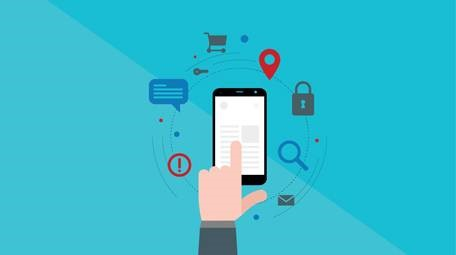
\includegraphics[width=0.8\linewidth]{description/framework/interactividad.jpg}
			\caption{Interactividad}
		\end{figure}
		\begin{center}
			\textbf{Fuente:} \url{https://kubik.mx/blog/category/mobile/}
		\end{center}
		}
	
		\subsubsection{Almacenamiento y persistencia de la información}
		
		{Los desarrollos tecnológicos en la informática y en la electrónica, han permitido que el almacenamiento de la información, pase de ser físico a digital, utilizando herramientas de almacenamiento en la nube para su posterior uso, conocidos como bases de datos, esto, facilitando la obtención de datos inmediatamente cuando son requeridos y garantizando el acceso a ellos.\\
			
		Las bases de datos, son un conjunto de datos almacenados en un medio informático que puede ser accedido por varios usuarios o aplicaciones a la vez, teniendo en cuenta como premisa, que estos no pueden ser redundantes e innecesarios.  \cite{angelData}.\\
		
		\begin{figure}[H]
			\centering
			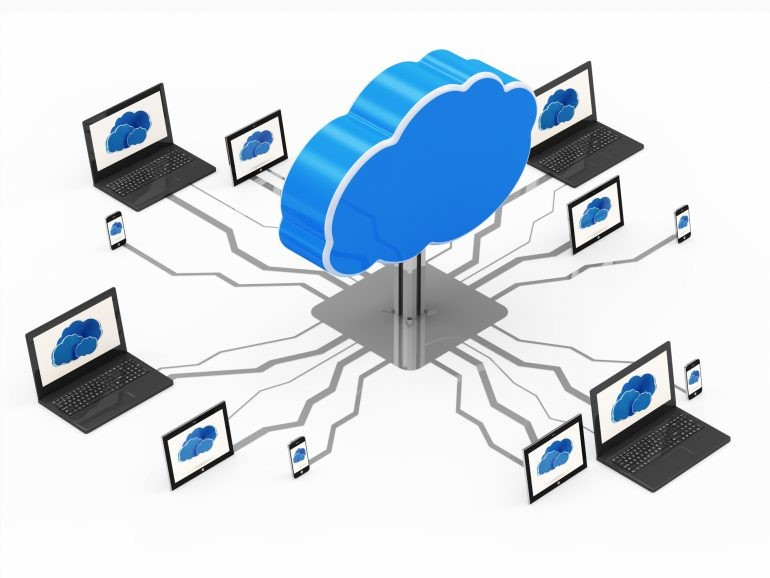
\includegraphics[width=0.8\linewidth]{description/framework/nube.jpg}
			\caption{Almacenamiento en la nube}
		\end{figure}
		\begin{center}
			\textbf{Fuente:} \url{https://smarterworkspaces.kyocera.es/blog/5-maneras-optimizar-la-rentabilidad-almacenamiento-la-nube/}
		\end{center}
	}
		
	
	\subsection{Marco Conceptual}
	
		\subsubsection{Sitios Web}
		
		{Un sitio web es un conjunto de archivos electrónicos y páginas web referentes a un tema en particular, incluyendo una página inicial de bienvenida generalmente denominada home page, a los cuales se puede acceder a través de un nombre de dominio y dirección en Internet específicos. El World Wide Web, o simplemente Web como se le llama comúnmente, está integrado por sitios web y éstos a su vez por páginas web. La gente suele confundir estos términos, pero un sitio web es en realidad un conjunto de páginas web.\\
			
		Los sitios web son empleados por las instituciones públicas y privadas, organizaciones e individuos para comunicarse con el mundo entero. En el caso particular de las empresas, este mensaje tiene que ver con la oferta de sus bienes y servicios a través de Internet, y en general para hacer eficiente sus funciones de mercadotecnia \cite{website}.
	
		\begin{figure}[H]
			\centering
			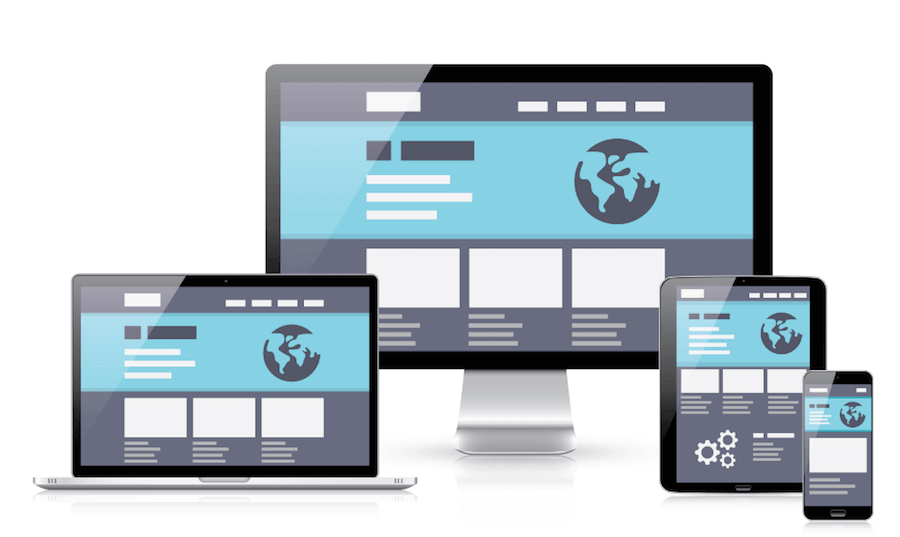
\includegraphics[width=0.8\linewidth]{description/framework/website.png}
			\caption{Sitio Web}
		\end{figure}
		\begin{center}
			\textbf{Fuente:} \url{https://informaticaydesarrollo.com/tag/diseno-de-paginas-web/}
		\end{center}
		}
		
		
		\subsubsection{Diseño Web responsive}
		
		{El diseño web responsive o adaptativo es una técnica de diseño web que busca la correcta visualización de una misma página en distintos dispositivos. Desde ordenadores de escritorio a tablets y móviles, en otras palabras, se trata de redimensionar y colocar los elementos de la web de forma que se adapten al ancho de cada dispositivo permitiendo una correcta visualización y una mejor experiencia de usuario. Se caracteriza porque los layouts (contenidos) e imágenes son fluidos y se usa código media-queries de CSS3 \cite{responsive}.\\
			
		El diseño responsive permite reducir el tiempo de desarrollo, evita los contenidos duplicados, y aumenta la viralidad de los contenidos ya que permite compartirlos de una forma mucho más rápida y natural.
	
		\begin{figure}[H]
			\centering
			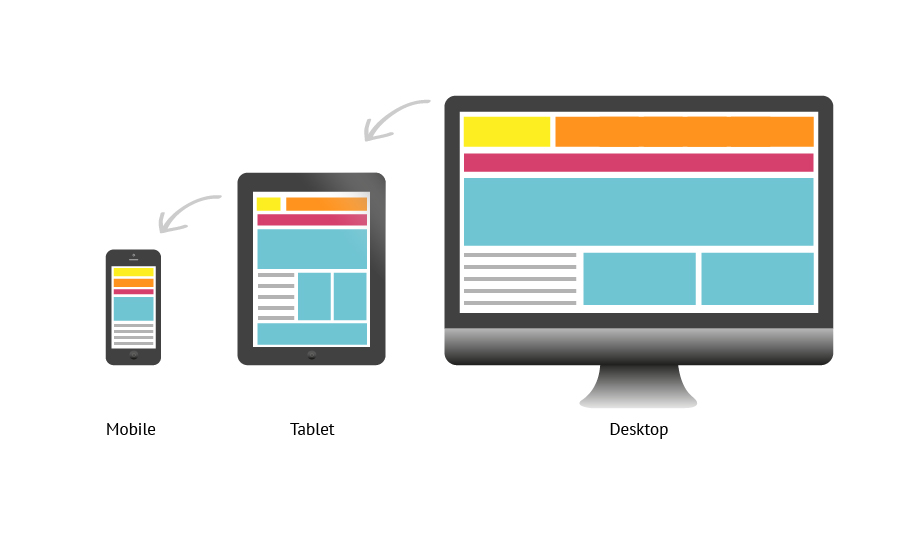
\includegraphics[width=0.8\linewidth]{description/framework/responsive.jpg}
			\caption{Diseño responsive}
		\end{figure}
		\begin{center}
			\textbf{Fuente:} \url{https://posicionamientoweb-seo.net/tips-para-lograr-un-diseno-web-responsive/}
		\end{center}
		}
			
		
		\subsubsection{Bases de datos relaciones}
		
		{Una base de datos relacional consiste en un conjunto de tablas, a cada una de las cuales se le asigna un nombre exclusivo, cada fila de la tabla representa una relación entre un conjunto de valores. De manera informal, cada tabla es un conjunto de entidades, y cada fila es una entidad, dado que cada tabla es un conjunto de tales relaciones, hay una fuerte correspondencia entre el concepto de tabla y el concepto matemático de relación, del que toma su nombre el modelo de datos relacional \cite{dataBase}.
		
		\begin{figure}[H]
			\centering
			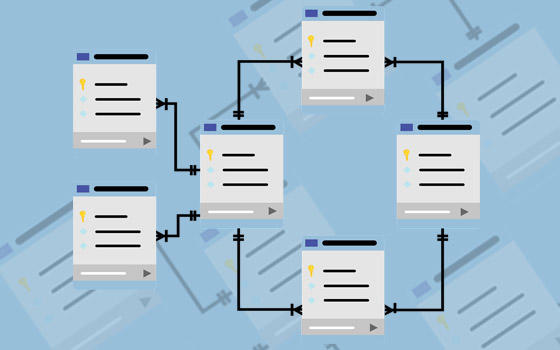
\includegraphics[width=0.8\linewidth]{description/framework/database.jpg}
			\caption{Bases de datos}
		\end{figure}
		\begin{center}
			\textbf{Fuente:} \url{https://www.aprendum.com.co/curso-virtual-administracion-gestion-bases-de-datos-sql/}
		\end{center}
		}
	
		\subsubsection{SQL}
		
		{El álgebra relacional proporciona una notación concisa y formal para la representación de las consultas. Sin embargo, los sistemas de bases de datos comerciales necesitan un lenguaje de consultas más cómodo para el usuario. SQL es un lenguaje de consultas distribuido comercialmente de más influencia. SQL usa una combinación de constructores del álgebra relacional y del cálculo relacional.\\
			
		Aunque se haga referencia al lenguaje SQL como “lenguaje de consultas”, puede hacer mucho más que consultar las bases de datos. Usando SQL es posible además definir la estructura de los datos, modificar los datos de la base de datos y especificar restricciones de seguridad \cite{dataBase}.\\
	
		No se pretende proporcionar un manual de usuario completo de SQL. En cambio, se presentan los constructores y conceptos fundamentales de SQL. Las distintas implementaciones de SQL pueden diferenciarse en detalles o admitir sólo un subconjunto del lenguaje completo.
	
		\begin{figure}[H]
			\centering
			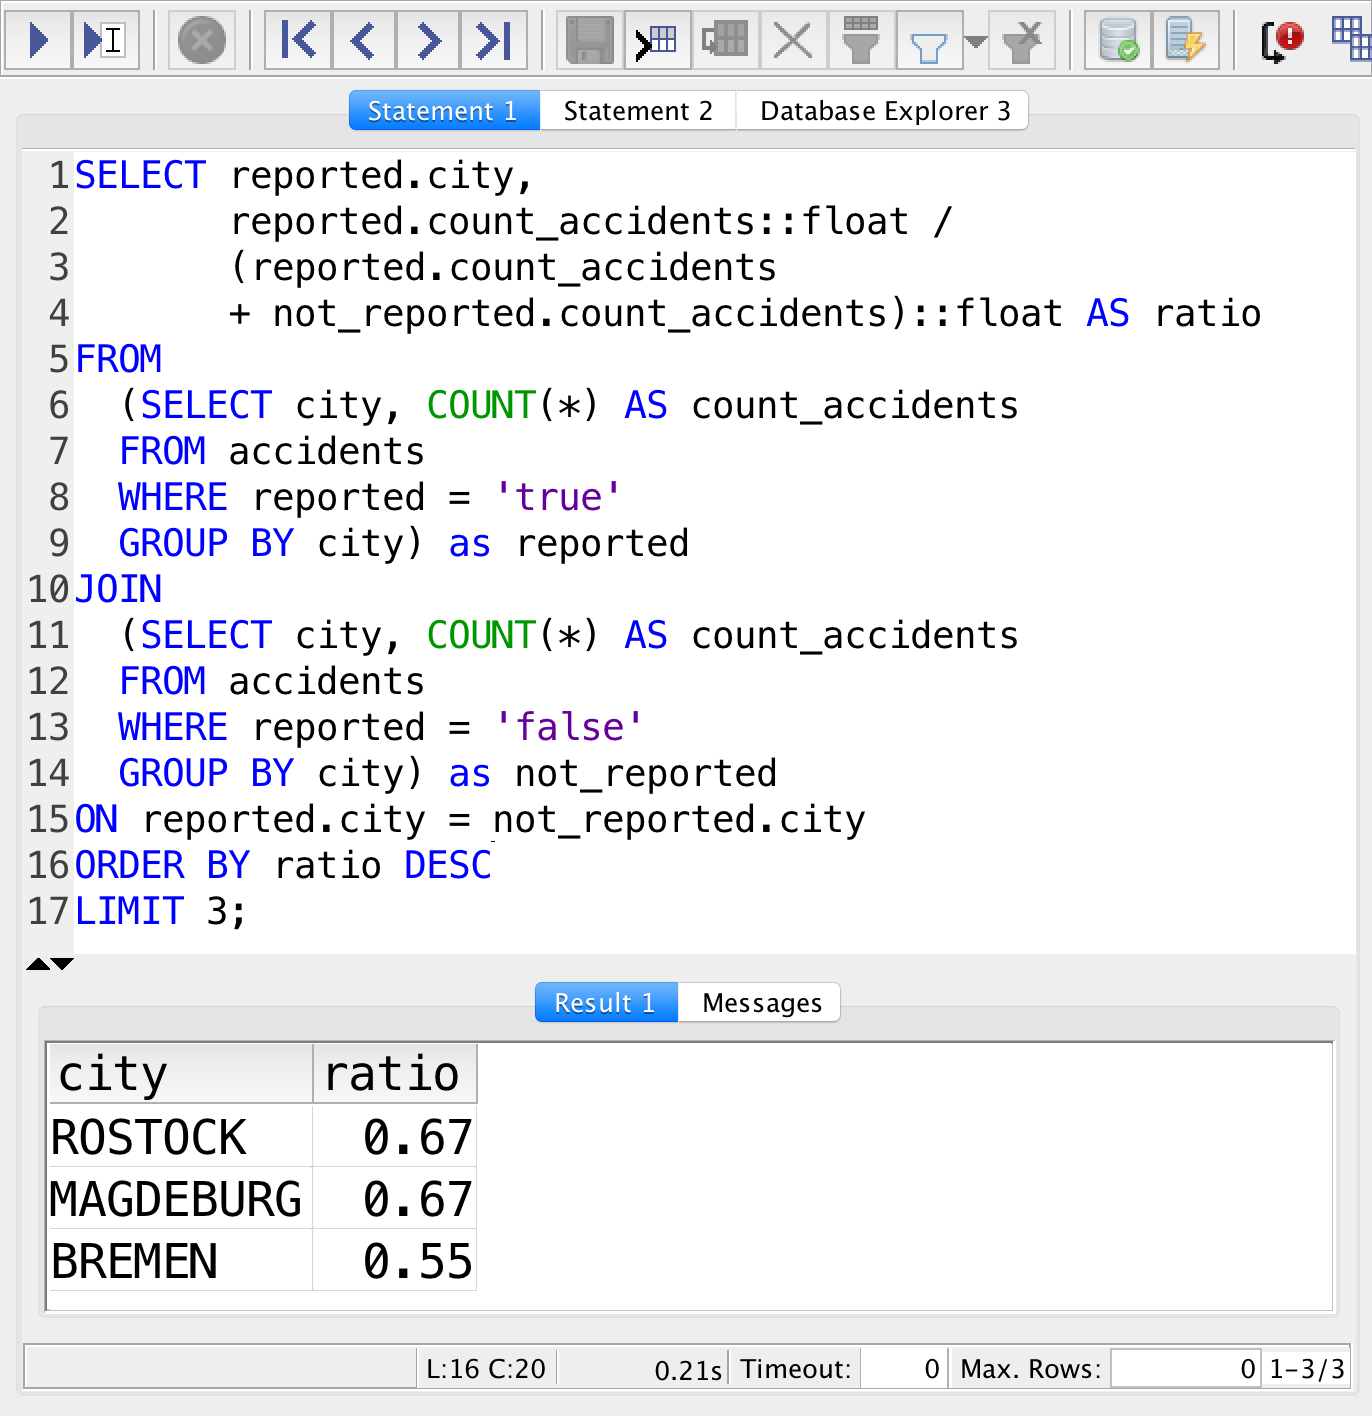
\includegraphics[width=0.6\linewidth]{description/framework/sql.png}
			\caption{sintaxis SQL}
		\end{figure}
		\begin{center}
			\textbf{Fuente:} \url{https://data36.com/sql-for-aspiring-data-scientists-7-day-online-course/}
		\end{center}
		}
	
	
		\subsubsection{RESTful}
		
		{La Transferencia de Estado Representacional (REST - Representational State Transfer) fue ganando amplia adopción en toda la web como una alternativa más simple a SOAP y a los servicios web basados en el lenguaje de descripción de servicios Web (Web Services Descripcion Language - WSDL). Ya varios grandes proveedores de Web 2.0 están migrando a esta tecnología, incluyendo a Yahoo, Google y Facebook, quienes marcaron como obsoletos a sus servicios SOAP y WSDL y pasaron a usar un modelo más fácil de usar, orientado a los recursos.\\
			
		REST define un set de principios arquitectónicos por los cuales se diseñan servicios web haciendo foco en los recursos del sistema, incluyendo cómo se accede al estado de dichos recursos y cómo se transfieren por HTTP hacia clientes escritos en diversos lenguajes. REST emergió en los últimos años como el modelo predominante para el diseño de servicios. De hecho, REST logró un impacto tan grande en la web que prácticamente logró desplazar a SOAP y las interfaces basadas en WSDL por tener un estilo bastante más simple de usar. \cite{restful}
		
		\begin{figure}[H]
			\centering
			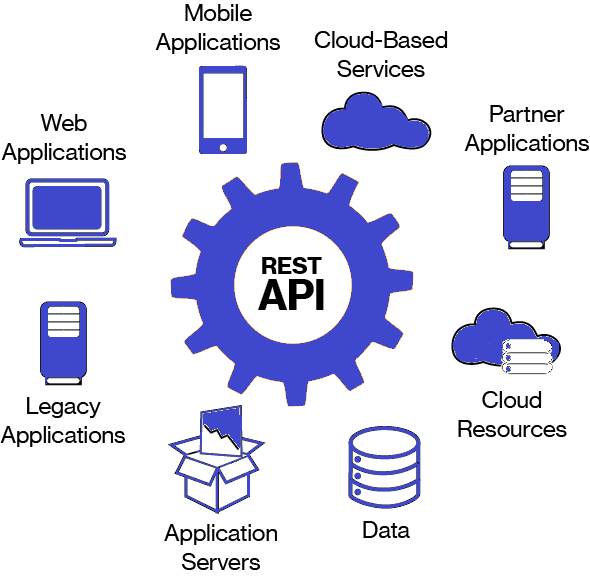
\includegraphics[width=0.6\linewidth]{description/framework/restful.png}
			\caption{Rest Api}
		\end{figure}
		\begin{center}
			\textbf{Fuente:} \url{http://www.gestclub.online/}
		\end{center}
		}
	
	
		\subsubsection{Web API}
		
		{Un Web API es un API que se invoca a través del protocolo HTTP. La ventaja de usar HTTP es que es posible hacer peticiones desde cualquier lenguaje de programación, lo que hace a la Web un medio ideal para conectar aplicaciones.\\
			
		Es posible encontrar Web API’s para casi cualquier cosa como: 
		
		\begin{itemize}
			\item Conocer el estado del tiempo.
			\item Conocer las tasas de cambio.
			\item Enviar emails.
			\item Recibir pagos.
			\item Entre miles de ejemplos más.
		\end{itemize}
			
		Muchos sitios y aplicaciones Web (Facebook, Twitter, Github, Trello, Google Maps, LinkedIn, Youtube, etc.) exponen gran parte de su funcionalidad a través de API’s permitiendo extender su funcionalidad en formas que ni los autores originales imaginaban (con el impacto positivo o negativo que eso implique) \cite{webapi}.
		
		\begin{figure}[H]
			\centering
			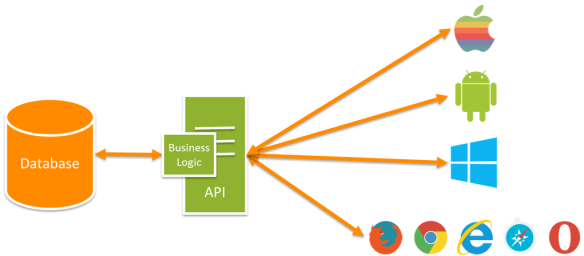
\includegraphics[width=0.8\linewidth]{description/framework/webapi.png}
			\caption{WEB API}
		\end{figure}
		\begin{center}
			\textbf{Fuente:} \url{https://techclub.tajamar.es/como-crear-una-web-api-y-acceder-a-datos-en-azure-usando-arquitectura-ado-net/}
		\end{center}
		}
		
		
		\subsubsection{HTTP}
		
		{Hypertext Transfer Protocol (HTTP) (o Protocolo de Transferencia de Hipertexto en español) es un protocolo de la capa de aplicación para la transmisión de documentos hipermedia, como HTML. Fue diseñado para la comunicación entre los navegadores y servidores web, aunque puede ser utilizado para otros propósitos también. Sigue el clásico modelo cliente-servidor, en el que un cliente establece una conexión, realizando una petición a un servidor y espera una respuesta del mismo. Se trata de un protocolo sin estado, lo que significa que el servidor no guarda ningún dato (estado) entre dos peticiones. Aunque en la mayoría de casos se basa en una conexión del tipo TCP/IP, puede ser usado sobre cualquier capa de transporte segura o de confianza, es decir, sobre cualquier protocolo que no pierda mensajes silenciosamente, tal como UDP \cite{http}.
		
		\begin{figure}[H]
			\centering
			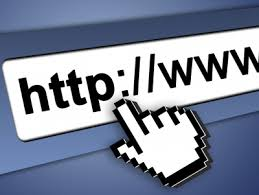
\includegraphics[width=0.7\linewidth]{description/framework/http.jpg}
			\caption{HTTP}
		\end{figure}
		\begin{center}
			\textbf{Fuente:} \url{https://seminariotcnico.wordpress.com/internet/}
		\end{center}
		}
			
